%%%%%%%%%%%%%%%%%%%%%%%%%%%%%%%%%%%
% RSC article draft
%%%%%%%%%%%%%%%%%%%%%%%%%%%%%%%%%%%

\documentclass[twoside,twocolumn,9pt]{article}
\usepackage{extsizes}
\usepackage[super,sort&compress,comma]{natbib}
\usepackage[version=3]{mhchem}
\usepackage[left=1.5cm,right=1.5cm,top=1.785cm,bottom=2.0cm]{geometry}
\usepackage{balance}
\usepackage{mathptmx}
\usepackage{sectsty}
\usepackage{graphicx}
\usepackage{lastpage}
\usepackage[format=plain,justification=justified,singlelinecheck=false,font={stretch=1.125,small,sf},labelfont=bf,labelsep=space]{caption}
\usepackage{float}
\usepackage{dblfloatfix}
\usepackage{fancyhdr}
\usepackage{fnpos}
\usepackage[english]{babel}
\addto{\captionsenglish}{\renewcommand{\refname}{Notes and references}}
\usepackage{array}
\usepackage{droidsans}
\usepackage{charter}
\usepackage[T1]{fontenc}
\usepackage[usenames,dvipsnames]{xcolor}
\usepackage{setspace}
\usepackage[compact]{titlesec}
\usepackage{hyperref}
\usepackage{orcidlink}
\usepackage{amsmath}
\usepackage{amssymb}
\usepackage{booktabs}
\usepackage{epstopdf}

\definecolor{cream}{RGB}{222,217,201}
\newcommand{\figureplaceholder}[2]{%
  \fbox{%
    \parbox[c][#2][c]{0.95\linewidth}{%
      \centering
      \textbf{Figure placeholder}\\[0.5ex]
      #1
    }%
  }%
}

\begin{document}
\pagestyle{fancy}
\thispagestyle{plain}
\fancypagestyle{plain}{\renewcommand{\headrulewidth}{0pt}}

\makeFNbottom
\makeatletter
\renewcommand\LARGE{\@setfontsize\LARGE{15pt}{17}}
\renewcommand\Large{\@setfontsize\Large{12pt}{14}}
\renewcommand\large{\@setfontsize\large{10pt}{12}}
\renewcommand\footnotesize{\@setfontsize\footnotesize{7pt}{10}}
\renewcommand\@biblabel[1]{#1}
\renewcommand\@makefntext[1]{\noindent\makebox[0pt][r]{\@thefnmark\,}#1}
\makeatother

\renewcommand{\thefootnote}{\fnsymbol{footnote}}
\renewcommand\footnoterule{\vspace*{1pt}\color{cream}\hrule width 3.5in height 0.4pt \color{black}\vspace*{5pt}}
\renewcommand{\figurename}{\small{Fig.}~}
\sectionfont{\sffamily\Large}
\subsectionfont{\normalsize}
\subsubsectionfont{\bf}
\setstretch{1.125}
\setlength{\skip\footins}{0.8cm}
\setlength{\footnotesep}{0.25cm}
\setlength{\jot}{10pt}
\titlespacing*{\section}{0pt}{4pt}{4pt}
\titlespacing*{\subsection}{0pt}{15pt}{1pt}
\fancyfoot{}
\fancyfoot[LO,RE]{\vspace{-7.1pt}
\includegraphics[height=9pt]{head_foot/LF}}
\fancyfoot[CO]{\vspace{-7.1pt}\hspace{13.2cm}
\includegraphics{head_foot/RF}}
\fancyfoot[CE]{\vspace{-7.2pt}\hspace{-14.2cm}
\includegraphics{head_foot/RF}}
\fancyfoot[RO]{\footnotesize{\sffamily{1--\pageref{LastPage} ~\textbar\hspace{2pt}\thepage}}}
\fancyfoot[LE]{\footnotesize{\sffamily{\thepage~\textbar\hspace{3.45cm} 1--\pageref{LastPage}}}}
\fancyhead{}
\renewcommand{\headrulewidth}{0pt}
\renewcommand{\footrulewidth}{0pt}
\setlength{\arrayrulewidth}{1pt}
\setlength{\columnsep}{6.5mm}
\setlength\bibsep{1pt}

\twocolumn[
\begin{@twocolumnfalse}
{
\includegraphics[height=30pt]{head_foot/journal_name}\hfill\raisebox{0pt}[0pt][0pt]{
\includegraphics[height=55pt]{head_foot/RSC_LOGO_CMYK}}\\[1ex]

\includegraphics[width=18.5cm]{head_foot/header_bar}}\par
\vspace{1em}
\sffamily
\begin{tabular}{m{4.5cm} p{13.5cm}}

\includegraphics{head_foot/DOI} & \noindent\LARGE{\textbf{Evaluating transfer across modalities in autonomous materials systems}} \\
\vspace{0.3cm} & \vspace{0.3cm} \\
 & \noindent\large{Kinston Ack{\"o}lf\,\orcidlink{0000-0002-5579-4878}$^{a}$ and Taylor D. Sparks\,\orcidlink{0000-0001-8020-7711}$^{*a}$} \\
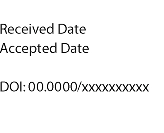
\includegraphics{head_foot/dates} & \noindent\normalsize{Autonomous materials workflows increasingly move between physical models, calibrated simulations, historical datasets, and machine-learning surrogates before decisions are validated in experiment or manufacturing. A central challenge is determining what knowledge remains reusable when the workflow representation changes. Here we introduce PyroEnGarde--Kintsugi (PEGKi), a framework for evaluating transfer across knowledge sources in autonomous materials systems. Using a controlled benchmark in which the nominal task is fixed while the underlying representation changes, we show that transfer is not a simple yes-or-no property. Instead, some forms of knowledge remain portable while others do not, and source usefulness depends on how a representation structures the accessible decision landscape. The results support a more philosophical view of autonomous materials design in which prior knowledge should be treated as partial, context-dependent, and diagnostically valuable rather than universally reusable. PEGKi is therefore best understood as a framework for source selection, transfer diagnosis, and trust in autonomous materials workflows.} \\
\end{tabular}
\end{@twocolumnfalse}\vspace{0.6cm}
]

\renewcommand*\rmdefault{bch}\normalfont\upshape
\rmfamily
\section*{}
\vspace{-1cm}

\footnotetext{\textit{$^{a}$Materials Science $\And$ Engineering, The University of Utah, 122 S. Central Campus Drive, Rm 304, Salt Lake City, Utah, USA 84112-0063. Corresponding author: Taylor D. Sparks. E-mail: taylor.sparks@utah.edu. Kinston Ack{\"o}lf publishes under this name and is also known as Kinston Wong. ORCiD: Kinston Ack{\"o}lf 0000-0002-5579-4878; Taylor D. Sparks 0000-0001-8020-7711.}}

\section{Introduction}

Consider a closed-loop thin-film workflow in which a controller must choose the next deposition temperature, gas ratio, or anneal after every measurement cycle. Early in the campaign, that choice might be guided by a transport model; later it might rely on a calibrated simulator, then on historical tool data, and finally on the measured film properties coming directly from the instrument. The target has not changed, for example maximising conductivity at a given thickness or steering the film toward a desired phase, but the representation of the search problem keeps changing as the workflow moves from model to surrogate to experiment. Autonomous materials science increasingly depends on workflows of exactly this kind that span more than one source of knowledge.\cite{Jain2013MaterialsProject,Kirklin2015OQMD,Dunn2020Matbench,Yoshida2025NetworkedAutonomous,Gongora2021SimulationTransfer} This layered workflow is useful because realism, cost, and speed are not identical. It also creates a practical question that is still weakly formalised: when several knowledge sources are available, what prior information or knowledge remains reusable, from which source, and with what level of trust?

For materials scientists, the key idea can be stated without specialised terminology. An \emph{autonomous materials system} is any workflow in which a model, rule, or controller repeatedly proposes the next material composition, process condition, or experiment on the basis of previous results. For example, a closed-loop thin-film deposition system that selects the next temperature and gas flow after each measured film property is an autonomous materials system. A \emph{source modality} is simply the kind of knowledge used to guide that decision, such as a first-principles model, a calibrated empirical model, a historical dataset, a heuristic rule set, or a machine-learning surrogate. For example, a density-functional-theory calculation, a measured sputtering archive, and a Gaussian-process surrogate are three different source modalities for the same design problem. \emph{Transfer} means reusing what was learned from one source modality after moving to another. For example, if a search strategy learned on simulation is reused to guide real experiments, that is transfer. The central question of this paper is whether the same guidance remains useful after that move, and if not, what part of the guidance still survives.

This question is related to, but not identical with, standard multi-fidelity modelling. Multi-fidelity methods have shown that low- and high-fidelity information can be combined to improve prediction and optimisation,\cite{Pilania2016MultiFidelityCoKriging,Tran2020MFGP} but most of that literature focuses on property prediction, surrogate learning, or sample efficiency. The less settled question is whether the \emph{guidance itself} transfers: a workflow, policy, ranking, or recommendation that performs well in one representation may not remain reliable when physical assumptions, calibration bases, or geometric constraints change.

Several familiar failure modes show why a transfer-aware framework is needed. Dataset aggregation in materials informatics can fail when coverage and calibration basis differ, so that adding more data does not necessarily add more usable structure.\cite{Ottomano2024DataAggregation} Code-to-code reproducibility studies show that even nominally equivalent computational pipelines can disagree in ways that matter for downstream decisions.\cite{Lejaeghere2016Reproducibility} Simulation-to-experiment studies show that one source can dramatically accelerate search in one setting while becoming misleading in another.\cite{Gongora2021SimulationTransfer} An analogous issue appears even in routine characterization: Vickers, Brinell, and Rockwell tests all probe hardness, yet they are related rather than interchangeable because their geometries and protocols differ.\cite{Broitman2017HardnessOverview} In each case, reuse cannot simply be assumed.

The practical need appears in several recognizable materials settings. In networked autonomous exploration, laboratories may wish to exchange learned priors or policy rankings across different target spaces.\cite{Yoshida2025NetworkedAutonomous} In simulation-assisted experimentation, one must decide whether a simulator, surrogate, or experimental archive should provide the initial prior for a scarce closed-loop campaign.\cite{Gongora2021SimulationTransfer} In crystal-structure prediction and inverse design, heuristic search, generative machine learning, and physics-based relaxation may all coexist, raising the question of which source is trustworthy for proposing candidates and which is trustworthy for evaluating them.\cite{Collins2025FUSE} Scientific infrastructures have improved FAIR data, interoperability, and machine-actionable metadata,\cite{Wilkinson2016FAIR,Andersen2021OPTIMADE,Ghiringhelli2023SharedMetadata} but optimisation results are still commonly reported as single-environment leaderboards. Such reports say little about whether a strong result should be reused, discounted, or ignored after a representation shift.

PEGKi is aimed at that decision layer. In an autonomous setting, the useful reusable unit is often not a raw model output but a transfer object: a ranking, uncertainty estimate, coverage statement, or routing rule that can survive movement into a different setting.

\begin{figure}
    \centering
    \includegraphics[width=\linewidth]{figures/figure1}
    \caption{Problem statement for cross-modality transfer in autonomous materials systems. One nominal design objective is pursued across multiple source modalities, including simulation, surrogate or machine-learning models, and experiment or measured data. The central question is what knowledge remains reusable after the representation changes.}
    \label{fig:problem_statement}
\end{figure}

Figure~\ref{fig:problem_statement} frames the core paper setting: one target objective, several representations of that objective, and a representation shift that may preserve some kinds of guidance while breaking others. In this work, we introduce PyroEnGarde--Kintsugi (PEGKi), a transfer-theoretic evaluation framework for autonomous materials systems under cross-modality shift. PEGKi represents the transfer problem in reduced form as
\[
\mathrm{AMS}=(K,A,D,R),
\]
where $K$ is a source representation or knowledge source, $A$ is a workflow controller or action-generating mechanism, $D$ is the deployment setting, and $R$ is the source-selection or source-routing mechanism. For the full closed-loop system, PEGKi uses
\[
\mathrm{AMS}=(K,A,D,O,U),
\]
where $O$ denotes observations returned by the material system and $U$ denotes the update rule that converts those observations into the next workflow step. Within that framework, PEGKi separates transfer into three levels: workflow-level transfer, relational transfer, and formulation-level transfer. This distinction is the core conceptual move of the paper. Transfer is not treated as a yes-or-no property, but as a structured diagnostic question.

These terms are meant in a practical materials-science sense. \emph{Workflow-level transfer} asks whether the same general way of running the materials workflow remains effective after the source modality changes. For example, in an XRD-guided workflow the raw diffraction pattern, the peak-fitting or refinement step, and the decision about the next synthesis or measurement are different parts of one process. If the same overall procedure for interpreting the pattern and choosing the next step remains useful after the data source or representation changes, that is workflow-level transfer. \emph{Relational transfer} asks whether the pattern of which methods tend to outperform or complement which other methods is preserved. For example, if one fitting-and-decision workflow remains more reliable than another across both simulated and measured diffraction data, that is relational transfer. \emph{Formulation-level transfer} asks the hardest question: if one source suggests a specific composition or process setting for a specific target, does that recommendation still work after moving to a different source modality? For example, if one workflow recommends one exact precursor ratio, annealing schedule, or measurement condition, formulation-level transfer asks whether that same recommendation still works after the representation changes. PEGKi was designed to separate these three questions because, in real materials work, they need not have the same answer.

The specific aims of this study are therefore fourfold: to define a compact framework for source-aware transfer in autonomous materials systems, to construct a controlled benchmark in which the nominal design task is fixed while the source modality changes, to test whether policy rankings and formulation-level recommendations transfer to the same degree, and to determine whether robust source reuse is better framed as single-source selection or mixed-source routing.

The same transfer problem appears across a broad class of materials workflows. A thin-film process may be described one way by a transport model, another way by historical tool data, and a third way by an ML surrogate. A battery optimisation loop may combine electrochemical measurements, degradation models, and empirical operating heuristics. A crystal-discovery workflow may move among heuristics, learned proposal models, and first-principles relaxation. In each case the nominal objective is shared, but the actionable landscape changes with the source modality.\cite{Gongora2021SimulationTransfer,Yoshida2025NetworkedAutonomous,Collins2025FUSE}

The present study focuses on that transfer question rather than on any one specific materials class. The benchmark choice is described in the Experimental section; the important point for the introduction is that the paper asks what remains reusable when the workflow context changes, even though the nominal task label stays the same. Figure~\ref{fig:concept} makes the paper's practical contribution explicit by showing where PEGKi enters an otherwise standard benchmark workflow.

Color matching is a useful entry point because it has already appeared in the self-driving-laboratory literature as both a simple closed-loop benchmark and a low-cost ``frugal twin'' for more expensive autonomous discovery platforms.\cite{Baird2023CLSLabLight,Ginsburg2023ExploringBenchmarks,Lo2024FrugalTwin} Liquid dye-based SDL demonstrations are conceptually closest to the Beer--Lambert side of the present benchmark, whereas pigment-based autonomous color-matching systems are conceptually closer to the pigment-mixing side represented here by Kubelka--Munk-style and related formulations, although none of these prior systems is identical to the specific forward models used in PEGKi. The present study shares that practical motivation but asks a different scientific question: not whether a single autonomous color-matching loop can be executed, but what transfers when the same nominal task is represented through different forward models.

\begin{figure}
    \centering
    \includegraphics[width=\linewidth]{figures/figure2}
    \caption{Workflow view of PEGKi relative to a standard benchmark pipeline. A typical workflow defines source modalities, generates a matched target set, evaluates policies under a fixed trial budget, and records outcomes. PEGKi then adds a transfer-analysis layer by constructing pairwise comparisons on matched targets, scoring policies, and diagnosing what knowledge is portable across modalities.}
    \label{fig:concept}
\end{figure}

\section{Experimental}

\subsection{Benchmark rationale}

To make the transfer question experimentally manageable, we use inverse color matching as a compact but chemically interpretable analogue of a materials workflow problem. The same formulation variables and the same target outcome are used across multiple color-mixing modalities, yet identical nominal inputs do not produce identical outputs because each modality embeds different physical assumptions, calibration data, reachable regions of design space, and latent constraints. This is exactly the kind of context shift that recurs throughout autonomous materials workflows: the nominal task is the same, but the operational landscape has changed.

This choice is also consistent with prior SDL work. Ginsburg \emph{et al.} use color matching as a flexible autonomous benchmark because it combines proposal, sample creation, and analysis in a single closed loop,\cite{Ginsburg2023ExploringBenchmarks} while Lo \emph{et al.} identify color-mixing SDLs as low-cost ``frugal twins'' for more expensive research systems.\cite{Lo2024FrugalTwin} PEGKi adopts the same general task for a different purpose: not to benchmark one liquid-handling platform, but to compare how knowledge transfers across alternative representations of the same task.

This comparison is informative but requires qualification. In broad optical terms, liquid SDL color mixing is closer to the transmission-style Beer--Lambert end of the benchmark, while pigment-based SDL color matching is closer to the reflectance and pigment-mixture end represented here by Kubelka--Munk-style and related models. PEGKi does not assume that those SDL platforms are equivalent to the present modalities; rather, it treats them as neighboring examples that motivate why color matching is a credible transfer testbed.

The color benchmark is therefore not meant to trivialise the materials problem. It is meant to isolate one difficult part of it. By keeping the nominal task fixed while changing the mapping from formulation to output, the benchmark makes it possible to ask a clean question: what survives when the context changes? In a synthesis, deposition, or scale-up problem, that same issue appears when identical nominal settings produce different outcomes because of drift, hidden variables, calibration differences, or different reachable process windows. The color benchmark provides a controlled way to study that transfer problem before moving to a full experimental platform.

The PEGKi demonstration uses a four-component color-mixture problem,
\[
(R,Y,B,W)\in\mathbb{R}_{\ge 0}^4,\qquad R+Y+B+W=100,
\]
where $R$, $Y$, $B$, and $W$ denote a shared four-coordinate mixture representation. In the Beer--Lambert modality, these coordinates correspond directly to the percentages of FD\&C Red 40, FD\&C Yellow 5, FD\&C Blue 1, and water, respectively, where FD\&C denotes certified U.S. Food, Drug, and Cosmetic food colorants. In the other modalities, the same coordinates play an analogous rather than identical role: KM maps them to the closest available red, yellow, blue, and white oil-pigment endpoints in the measured K/S database; MB treats them as digital pigment-mixture inputs with a white endpoint; and RYB treats them as digital red-yellow-blue artist-theory inputs diluted toward white. All candidate formulations were represented in continuous composition space and evaluated as color outputs on a 0--255 RGB (red-green-blue) scale.

More generally, each source modality $K_j$ defines its own forward map
\[
f_j:\mathcal{X}\rightarrow \mathcal{Y}_j,
\]
from the shared composition space $\mathcal{X}$ to a modality-specific response space $\mathcal{Y}_j$. The inverse-design task for target color $y^\ast$ is therefore
\[
x^\ast_j \in \arg\min_{x\in\mathcal{X}} d\!\left(f_j(x),y^\ast\right),
\]
with the same nominal design variables and target across all modalities, but with a different contextual map $f_j$ in each case.

This domain is useful because it is continuous, compositional, constrained, and easy to express through multiple distinct source modalities while holding the nominal task fixed. The benchmark therefore compresses a general autonomous-materials problem into a controlled setting: the same nominal inputs and the same nominal target, but different contextual maps from formulation to outcome.

\subsection{Base modalities and derived datasets}

\begin{figure}
    \centering
    \includegraphics[width=\linewidth]{figures/modality_overlay_rgb_3d}
    \caption{Four base modalities overlaid in RGB space using the shared four-component formulation representation. BL, KM, MB, and RYB occupy overlapping but non-identical regions of accessible color space, illustrating that the same nominal inverse-design task is expressed through different reachable landscapes before any transfer analysis is performed.}
    \label{fig:benchmark_design}
\end{figure}

PEGKi was demonstrated on four base modalities: a Beer--Lambert dye-absorption model (BL), a Mixbox surrogate pigment model (MB),\cite{Sochorova2021} a Kubelka--Munk measured-pigment model (KM) anchored to measured oil-pigment K/S (absorption-to-scattering) spectra,\cite{Kubelka1931,Wiersma2025Hyperspectral} and an artist RYB mixing model (RYB).\cite{Gossett2004RYB} The benchmark comprised seven datasets: four single-modality datasets and three cross-modality studies built from overlap or difference regions between modality pairs.

The four single-modality datasets correspond to the BL, MB, KM, and RYB modalities themselves. The three cross-modality studies represent the MB+RYB shared region, the BL$-$RYB difference region, and the KM$-$MB difference region. All datasets in the current benchmark were evaluated against a shared target pool so that cross-modality comparisons reflected the same nominal design task under different representations, analogous to targeting the same materials objective across different knowledge sources or workflow stages.

This seven-dataset design is central to PEGKi. The four single-modality datasets say how policies behave within each modality. The overlap and difference datasets say what additional structure is shared, what structure is unique, and whether an apparent transfer advantage is geometrically meaningful or merely accidental. The current benchmark uses a shared pool of just over 100 achievable target colours sampled from modality outputs rather than from uniform RGB space, so every target is reachable by construction within the benchmark setting.
Figure~\ref{fig:benchmark_design} shows the same point geometrically: the modalities overlap, but they do not occupy identical accessible regions, so transfer is being tested under a real change in reachable landscape rather than under a trivial relabeling of one common space.

\subsection{Policy-evaluation protocol}

Nine optimisation policies were evaluated: grid search, simulated annealing, evolutionary strategy, Bayesian optimisation with expected improvement, Bayesian optimisation with upper confidence bound, UCB1 bandit, Thompson sampling, random forest, and a multilayer perceptron regressor. For each of the seven datasets, the shared target pool was optimised under a fixed budget of 50 sequential trials per target. At each trial, the policy proposed a composition, the selected modality returned the color response, and the policy was updated from the observed error.

Policies were evaluated independently against matched target sets, because the current benchmark is not a direct competitive multi-agent setting but a shared-target comparison setting. As a result, the main ranking signal is expected to be transitive at the strategy level, even if richer intransitive structure appears in auxiliary analyses.

The present study is computational. It uses pre-defined source modalities and benchmark targets and does not involve wet-lab procedures, additional chemical handling, or special experimental hazards. All analysis was performed on saved benchmark outputs and transfer-analysis files, so the workflow is reproducible from the project configuration, rating outputs, shared target file, and transfer-analysis artefacts described in the accompanying technical reference.

\subsection{Performance, rating, and transfer}

The primary response was the best color error achieved within an experiment,
\[
d_i=\min_t \frac{|R_t-R^\ast|+|G_t-G^\ast|+|B_t-B^\ast|}{3},
\]
where lower values indicate better target matching. This metric is benchmark-specific: it is the objective used to compare policies on a shared inverse-design task, not a claim that RGB error is a universal materials metric. PEGKi converted policy outcomes into post hoc pairwise comparisons on matched targets and then estimated Bayesian skill ratings using a TrueSkill-style framework.\cite{Herbrich2006TrueSkill} TrueSkill is the only reader-facing $\mu,\sigma$ leaderboard used in the present manuscript. The remaining models were retained for structural diagnostics in their native forms, such as antisymmetric matchup structure, Hodge-style decomposition, latent ranking contexts, and cyclic-subgame supports, because policies were assessed independently against common targets.

Cross-modality transfer was analyzed through the directional score
\[
\Delta(K_s \rightarrow K_t)=
\lambda_{\sigma}\,\sigma(K_s,K_t)+
\lambda_{\rho}\,\rho(K_s,K_t)-
\lambda_{\omega}\,\omega(K_s,K_t),
\]
where $\sigma$ is a structural-compatibility term, $\rho$ is a mapping-efficiency term derived from cross-modality rank agreement, and $\omega$ is a transfer-overhead term that penalizes target-only degradation. In the current benchmark, the source-quality term was removed because absolute rating level is engine-local and not comparable across modalities, and the remaining weights were fixed at $(\lambda_{\sigma},\lambda_{\rho},\lambda_{\omega})=(1.0,1.0,1.0)$ rather than learned from data. $\Delta$ is therefore an operational source-selection score rather than a universal physical quantity. Its present limitation is that the weighting is hand-specified rather than learned; a larger benchmark with labelled successful and unsuccessful transfers could instead fit these weights, or a richer transfer predictor, directly from observed transfer outcomes.

To turn pairwise transfer scores into a practical source-selection rule, PEGKi uses a mixed-source routing problem over the source simplex:
\[
r^\ast \in \arg\max_{r\in \Delta^{m-1}} \min_{t} \sum_{s=1}^{m} r_s\,\Delta(K_s\rightarrow K_t),
\]
where $r_s$ is the allocation weight on source $K_s$ and $\Delta^{m-1}$ denotes the probability simplex over the $m$ candidate sources, that is, all non-negative source weights that sum to one. This is the paper-level expression of the Nash-style routing analysis reported in the technical reference: a robust prior is chosen by maximizing worst-case transfer utility across targets.

\begin{table*}[!t]
\small
\caption{\ PEGKi study matrix. BL = Beer--Lambert, MB = Mixbox, KM = Kubelka--Munk, and RYB = artist RYB.}
\label{tab:study_matrix}
\begin{tabular*}{\textwidth}{@{\extracolsep{\fill}}p{0.11\textwidth}p{0.22\textwidth}p{0.18\textwidth}p{0.35\textwidth}}
\hline
\textbf{Label} & \textbf{Source modality} & \textbf{Study type} & \textbf{Why it is included}\\
\hline
BL & Beer--Lambert & Single modality & Reference dye-absorption modality\\
MB & Mixbox & Single modality & Fast surrogate pigment modality\\
KM & Kubelka--Munk & Single modality & Measured-pigment modality\\
RYB & Artist RYB mixing & Single modality & Heuristic artist-theory modality\\
MB+RYB & Mixbox + RYB & Overlap region & Tests agreement and redundancy in a shared region\\
BL$-$RYB & Beer--Lambert relative to RYB & Difference region & Tests representation asymmetry\\
KM$-$MB & Kubelka--Munk relative to Mixbox & Difference region & Tests material and calibration asymmetry\\
\hline
\end{tabular*}
\end{table*}

\section{Results and discussion}

\subsection{How to read the results}

Interpretation of the benchmark requires separating three questions. Each method is given the same task: start from the same target colour, make up to 50 sequential formulation proposals, and try to reach the target as closely as possible within one source modality. The source modality is then changed while the nominal task stays the same. The first question is whether the same methods remain strong after that change. The second question is whether the relationships among methods remain similar. The third question is whether a specific formulation recommendation survives the change. These are the three levels of transfer used throughout the paper.

Two distinctions are especially important. First, a method can transfer well at the workflow level even if it does not transfer well at the formulation level. A source can therefore remain informative about \emph{how to run the search} even when it does not correctly predict \emph{the exact answer}. Second, agreement in a shared part of design space does not guarantee agreement everywhere. Two source modalities may appear similar where both can represent the target, but diverge strongly once one modality reaches regions the other cannot represent. The overlap and difference datasets were designed specifically to expose that distinction.

\subsection{A stable strategy hierarchy appears across modalities}

The seven-dataset benchmark produces a clear and remarkably stable method hierarchy. Bayesian UCB is the top-ranked generalist under the present protocol, ranking first in all seven datasets. Bayesian expected improvement forms a strong second tier. Evolutionary Strategy and Simulated Annealing remain consistently competitive while operating at much lower computational cost, making them the strongest quality--cost compromise in the present study. In the current runs, Bayesian optimisation typically required on the order of $10^4$ s per dataset, whereas evolutionary strategy and simulated annealing completed in only a few seconds and simpler baselines such as grid search, UCB1, and random forest generally remained in the tens-to-low-hundreds-of-seconds range. The ranking should therefore be read as a performance ordering under the benchmark protocol rather than as a universal statement of practical preference: computational cost is distinct from transferability, but it strongly affects which transferable workflow is attractive in deployment. This is the main workflow-level result of the paper: the benchmark identifies a stable ordering of decision methods rather than a different winner for each modality.

The benchmark does not imply that one exact composition transfers everywhere. It shows instead that certain ways of running an adaptive search remain broadly reliable even when the source modality changes. In the current study, uncertainty-aware Bayesian search defines the highest-performing workflow tier under the present metric, while evolutionary and annealing-style workflows may be the more practical choices when computational cost matters.

This stability is operationally useful. In many real workflows, one first needs to decide what kind of closed-loop procedure should be trusted before deciding what specific prior should be reused. The present ranking result says that the benchmark is stable enough to support that kind of workflow-level comparison.
Figure~\ref{fig:policy_summary} gives a representative example of that stability in the BL dataset and illustrates the publication-facing TrueSkill ranking used throughout the manuscript.

\begin{figure*}
    \centering
    \includegraphics[width=0.76\textwidth]{figures/policy_summary_bl_ts}
    \caption{Representative TrueSkill policy ranking for the BL dataset. Error bars denote posterior uncertainty on the global skill axis. Bayesian UCB and Bayesian expected improvement define the strongest tier, while evolutionary strategy and simulated annealing remain competitive at lower complexity; the same broad ordering pattern persists across the remaining benchmark datasets.}
    \label{fig:policy_summary}
\end{figure*}

\subsection{The benchmark is transitive at the strategy level}

The present PEGKi benchmark is dominated by transitive ranking. Under the current evaluation design, methods are compared on common benchmark targets after execution rather than interacting directly during search. The benchmark therefore measures global workflow quality rather than opponent-specific cyclical dominance. This result is important for interpreting PEGKi correctly: the framework can host richer intransitivity-aware components, but those components are not automatically informative in every benchmark design.

The same distinction is relevant to prior work as well. PEGKi borrows useful tools from rating and empirical game analysis, but the present benchmark should not be read as evidence for rich cyclic competition among optimisers. Its main value is instead the transfer diagnosis made possible by shared-target comparisons across source modalities.

Accordingly, the rankings should be interpreted in the usual sense: methods near the top are broadly stronger across the benchmark than methods near the bottom. The point of the more advanced rating machinery is not to replace that intuition, but to test whether the same ordering is preserved under source change and to quantify where that ordering starts to break down.

\subsection{Strategy-level knowledge transfers more reliably than formulation-level guidance}

The main transfer result follows directly from the stability above. Workflow-level guidance is more portable than formulation-level guidance. Across the seven datasets, the same methods remain near the top of the ranking even when the modality changes. By contrast, target-specific formulation advice does not transfer comparably well. Quantitatively, the shared relational component is substantial but incomplete ($0.647$), whereas the mean per-target trajectory correlation is only $0.029$. A source modality may therefore be useful for choosing \emph{how} to run a search or screening workflow even when it is not reliable for predicting \emph{what exact formulation} should be used after transfer.

This difference is central to the paper. Suppose one source modality tells a researcher that uncertainty-aware adaptive search is a good way to explore a new materials problem. That lesson may still hold after moving to a different source modality. But if the same source recommends one exact precursor ratio, one exact layer order, or one exact annealing setting, that concrete recommendation may fail after transfer because the second modality maps inputs to outputs differently. PEGKi shows that these two kinds of reuse should not be treated as the same thing.

The benchmark numbers support that interpretation directly. A shared relational component of $0.647$ means that a meaningful fraction of the \emph{method structure} is common across modalities, but not all of it. A very low formulation-level trajectory correlation means that \emph{target-by-target recommendations} are not common in the same way. The framework therefore gives a more precise answer than simply saying that transfer works or does not work.

\subsection{Transfer is directional rather than interchangeable}

\begin{figure}
    \centering
    \includegraphics[width=\linewidth]{figures/transfer_delta}

    \vspace{0.4em}
    \includegraphics[width=\linewidth]{figures/donor_strength}
    \caption{Directional transfer and source usefulness in PEGKi. Top: the ordered transfer matrix $\Delta(K_s \rightarrow K_t)$ for all source-target pairs. Bottom: aggregate source usefulness, showing outgoing transfer score, asymmetry advantage, Spearman agreement, and the Nash routing weights. In both panels, modalities are listed in the same top-to-bottom order: BL, MB, KM, RYB, MB+RYB, BL$-$RYB, and KM$-$MB. Together these outputs show that transfer is directional and that the most robust prior is mixed rather than single-source.}
    \label{fig:transfer_summary}
\end{figure}

Transfer across datasets is directional rather than interchangeable. Source quality is strongly non-uniform across the 42 ordered source-target pairs in the current benchmark. In the current run, the most robust prior is not a single dataset but a weighted mixture dominated by KM ($0.386$), the MB+RYB shared-region dataset ($0.377$), and the KM$-$MB difference dataset ($0.236$). By contrast, BL is a useful target but a weak source for other modalities. The transfer landscape is therefore not governed by a single universal ordering.

Here, ``directional'' means that a source that helps when moving from A to B need not help equally when moving from B to A. This is familiar in materials practice: knowledge that is useful when moving from a simplified model toward a calibrated process does not necessarily move cleanly in the reverse direction. PEGKi makes that asymmetry measurable rather than leaving it as intuition.

The mixed-source result strengthens that point. If one source dominated everywhere, transfer could be treated as a simple winner-takes-all problem. That is not what happens here. Instead, different sources contribute different kinds of useful structure, so the most robust reuse strategy is a weighted combination rather than a single trusted source.
These directional and aggregate donor effects are summarized visually in Figure~\ref{fig:transfer_summary}.

\subsection{Overlap and difference datasets explain why asymmetry appears}

\begin{figure}
    \centering
    \includegraphics[width=\linewidth]{figures/asymmetry_heatmap}
    \caption{Transfer asymmetry heatmap in PEGKi. The dominance ratio indicates which source is stronger for a given ordered pair, and blue borders mark modality pairs with verified asymmetry. This diagnostic emphasizes that transfer is directional rather than interchangeable across source-target pairs.}
    \label{fig:transfer_diagnostics}
\end{figure}

The overlap and difference studies reveal that PEGKi detects more than one kind of asymmetry. In the BL$-$RYB case, self-domain advantage is positive and coherent: the BL modality retains an advantage on colors that the RYB manifold cannot represent. In the KM$-$MB case, self-domain advantage is also positive, but the policy-proximity diagnostic is strongly incoherent. KM therefore shows some local ownership of its exclusive region without supplying a stable transferable regime across policies.

This feature is important because the single-modality datasets tell us that asymmetry exists, whereas the overlap and difference datasets identify what kind of asymmetry it is. Some asymmetries arise because one modality contains structure the other cannot represent. Others arise because a measured or calibrated source is narrower than expected and does not export its knowledge well even into regions it uniquely occupies.

This distinction is important because not all failure modes mean the same thing. If one modality wins on its own unique region and does so coherently across policies, that suggests real domain ownership: the source contains useful structure the comparison source lacks. If the same region is only weakly favourable or behaves incoherently across policies, the implication is different. The source may still encode useful local structure, but it is too narrow, too brittle, or too extrapolative to trust as a stable donor. PEGKi therefore turns ``these two sources disagree'' into a more informative diagnosis of \emph{why} they disagree.
Figure~\ref{fig:transfer_diagnostics} shows that asymmetry pair-by-pair and helps distinguish simple source superiority from genuinely directional transfer structure.

\subsection{Calibration basis matters more than nominal physical rigor}

The most counterintuitive result in the current benchmark is that nominal physical rigor does not by itself determine source usefulness. The Beer--Lambert modality is the most first-principles-like model in the set, but it is not the strongest transfer source. By contrast, the materially calibrated KM modality and the overlap/difference datasets derived from it provide the most robust transfer routes. This supports a central PEGKi claim: source usefulness depends more on calibration basis and actionable structure than on nominal physical sophistication. In that sense PEGKi extends the lesson already visible in aggregation, reproducibility, and simulation-transfer studies: source quality is not exhausted by nominal fidelity alone.\cite{Ottomano2024DataAggregation,Lejaeghere2016Reproducibility,Gongora2021SimulationTransfer,Yoshida2025NetworkedAutonomous,Collins2025FUSE}

This point is likely to resonate with materials scientists because it matches common experience. A nominally more physical model is not always the most useful model for guiding the next real decision. A calibrated source that better reflects the actual reachable process space may be more valuable than a cleaner but less well-matched theory model. PEGKi does not argue against first-principles modelling; it argues that transfer usefulness should be judged by what survives into the next workflow stage, not by prestige or nominal rigor alone.

\subsection{Mixed-source routing is more robust than single-source transfer}

Weighted source routing is more robust than single-source transfer. The resulting allocation is strongly non-uniform and, in the current run, mixed rather than pure. PEGKi is therefore not only a benchmark for who wins; it is a decision layer for which source or source mixture should guide the next optimisation step. In the current routing solution, all mass is placed on three sources and zero weight on the remaining four, which is a much sharper decision than simply saying that all source modalities are useful.

This feature most clearly differentiates PEGKi from a standard benchmarking paper. A leaderboard would stop at ``Bayesian UCB wins.'' PEGKi continues to ask which source should donate the prior, whether that source is safe to trust in the target setting, and whether a weighted combination is more robust than a single donor. The current answer is that a mixture is often safer than a pure choice.

A materials workflow often has access to more than one prior source: a simulator, an empirical archive, a heuristic rule set, or a learned surrogate. PEGKi suggests that the right question is not always ``Which single source is best?'' It may instead be ``Which combination of sources gives the safest and most useful guidance for the next stage?'' The present benchmark supports the second view.

\subsection{What this benchmark does and does not claim}

The present study remains a demonstration of PEGKi rather than a complete survey of autonomous-materials settings. The transfer scores are defined within the PEGKi formalism, the demonstration domain is color formulation, and the case studies reflect the geometry of the four modalities used here. PEGKi functions here as a theory and evaluation layer rather than as validated plant-scale process control. The current evidence comes from a computational benchmark of 7 datasets, 9 policies, a shared target pool of just over 100 colours, and 50-trial sequential runs; it does not yet include a closed-loop experimental validation on a real materials platform.

The benchmark is strong where autonomous materials systems need help deciding how to reuse prior knowledge: source selection, asymmetry diagnosis, coverage reasoning, and transfer routing. It is much weaker on direct experimental closure across real material systems, and it should not be read as a substitute for actual closed-loop simulation-to-experiment or lab-to-fab validation. Its contribution is instead to make the transfer problem itself legible.

Accordingly, the present manuscript is a benchmark and framework paper. The color-formulation setting is the demonstration domain, not the ultimate target application. The stronger claim is that PEGKi provides a principled language for asking which source to trust, which part of knowledge transfers, and how much of that transfer should be reused after a change in representation.

\subsection{Implications for autonomous materials science}

If the present interpretation continues to hold beyond the color-formulation benchmark, PEGKi suggests that autonomous materials science needs more than better optimizers. It also needs a transfer layer that decides what prior knowledge is portable, what level of abstraction is portable, and when disagreement among sources is itself informative. In that view, the reusable object in an autonomous workflow is not always a raw model or dataset. It may instead be a certified transfer object: a policy ranking, a coverage statement, a reliability score, or a source-routing rule that remains useful after a change in representation.\cite{Ottomano2024DataAggregation,Lejaeghere2016Reproducibility,Yoshida2025NetworkedAutonomous}

That future-facing interpretation is especially relevant for multi-lab systems and hybrid pipelines. A network of autonomous laboratories may need to share not just observations, but trustworthy priors.\cite{Yoshida2025NetworkedAutonomous} A simulation-assisted campaign may need to decide when to trust a fast surrogate, when to trust a measured archive, and when to hedge by combining them.\cite{Gongora2021SimulationTransfer} A hybrid inverse-design loop may need to route among heuristics, generative models, and physics-based evaluators rather than assuming that one source dominates globally.\cite{Collins2025FUSE} PEGKi does not yet prove that this transfer layer is universally sufficient, but it provides a concrete framework for asking those questions in a way that can be benchmarked and eventually validated on real materials systems.

\section*{Conclusions}

PEGKi introduces a way to evaluate transfer across heterogeneous source modalities in autonomous materials systems. The main contribution is not a new colour model or a new optimiser. It is a framework for deciding what kind of prior knowledge remains useful after a change in representation.

The present benchmark supports four linked interpretations. First, transfer is directional rather than interchangeable. Second, strategy-level guidance is more portable than formulation-level guidance. Third, calibration basis matters more than nominal physical rigor for source usefulness. Fourth, robust source choice is often mixed rather than single-source. These results also separate benchmark ranking from practical preference: a high-performing transferable workflow is not automatically the most attractive deployment choice once decision cost is considered. Together these points shift the problem from simple benchmarking toward source selection, transfer diagnosis, and trust.

The broader significance is practical. If autonomous materials workflows continue to combine physics models, empirical datasets, machine-learning surrogates, and experimental measurements, they will need a principled way to decide what knowledge is portable and what knowledge is not. Future work should test PEGKi on real closed-loop materials systems and determine whether the same transfer structure persists in simulation-to-experiment and lab-to-manufacturing settings.

\section*{Author contributions}
Kinston Ack{\"o}lf: Conceptualization, Methodology, Software, Formal analysis, Investigation, Visualization, Writing--original draft, Writing--review \& editing. Taylor D. Sparks: Supervision, Writing--review \& editing.

\section*{Conflicts of interest}
There are no conflicts to declare.

\section*{Data availability}
The code, benchmark configuration, shared target set, trained-rating outputs, and transfer-analysis outputs that support this study will be made available on GitHub in the PEGKi project repository. The technical details of the workflow and the traceability layer for the reported results are documented in the accompanying technical reference.

\section*{Acknowledgements}
The authors acknowledge discussions within the University of Utah materials-science research environment that informed the development of PEGKi.

\bibliography{rsc}
\bibliographystyle{rsc}

\clearpage
\appendix
\section{Annex: Extended framework and supplementary notes}

This annex collects the mathematical, methodological, and interpretive material that supports the core manuscript but would otherwise interrupt the main narrative. It is intended to play the role of an integrated annex and supplementary note. The goal is not to repeat every line of the project technical reference verbatim, but to preserve the main framework, definitions, derivations, and traceability structure in manuscript form.

\subsection{Abbreviations and naming}

The four source modalities are Beer--Lambert dye-absorption (BL), Mixbox surrogate pigment (MB), Kubelka--Munk measured-pigment (KM), and artist RYB mixing (RYB).\cite{Kubelka1931,Sochorova2021,Gossett2004RYB,Wiersma2025Hyperspectral} Derived datasets are MB+RYB for the shared region between MB and RYB, BL$-$RYB for the BL-only region relative to RYB, and KM$-$MB for the KM-only region relative to MB. Rating abbreviations used in the extended PEGKi workflow include TrueSkill (TS), Blade--Chest (BC), Flow/Fredholm game decomposition (FFG/Hodge), Bayesian neural network (BNN), intransitive clustered Bradley--Terry (ICBT), and Spinning Tops (ST).\cite{Herbrich2006TrueSkill,ChenJoachims2016Intransitivity,Wellman2006EGTA,Czarnecki2020SpinningTop}

\subsection{Extended PEGKi framework}

PEGKi represents an autonomous-materials transfer problem in reduced form as
\[
\mathrm{AMS}=(K,A,D,R),
\]
and in full closed-loop form as
\[
\mathrm{AMS}=(K,A,D,O,U),
\]
where $K$ is the source representation or knowledge source, $A$ is the decision policy or action-generating mechanism, $D$ is the deployment setting, $R$ is the source-selection or source-routing mechanism, $O$ is the observation stream returned by the material system, and $U$ is the update rule mapping observations to the next action. In practice, these objects may be implemented as stages of a single pipeline rather than as separate software modules. For example, in an XRD-guided synthesis loop the raw diffraction pattern is naturally interpreted as $O$, the peak-finding or refinement routine is usually part of $U$, the refined feature representation may become part of $K$, and the controller selecting the next synthesis condition is $A$.

Within this framework PEGKi distinguishes three transfer levels:
\begin{enumerate}
\item strategy transfer, which asks whether the ordering of decision policies survives a change in source modality;
\item relational transfer, which asks whether pairwise dominance, complementarity, or cyclic structure survives;
\item formulation-level transfer, which asks whether target-specific recommendations survive unchanged.
\end{enumerate}

The current benchmark supports a layered answer rather than a binary one. Strategy-level information is comparatively stable, relational information is partially stable, and formulation-level guidance is weak. This layered view is one of the main conceptual claims of PEGKi.

\subsection{Working conjectures and their current status}

The PEGKi interpretation is organised around four working conjectures.

\textbf{Directional transfer predictability.} Transfer asymmetry is not random. It should be explainable from coverage mismatch, calibration basis, and changes in rank geometry between source and target.

\textbf{Information irreducibility of materials knowledge.} Some empirically grounded materials knowledge cannot be faithfully compressed into lower-fidelity or differently parameterised spaces without losing decision-relevant structure.

\textbf{Strategy--formulation separation.} Strategy-level and relational knowledge transfer more reliably than formulation-level recommendations.

\textbf{Mixed-source optimality under shift.} Under cross-modality shift, the most robust prior is often a weighted combination of sources rather than a single globally dominant source.

In the current benchmark, the third and fourth conjectures are strongly supported, the first is supported in a benchmark-specific sense, and the second is partially supported. These should be read as benchmark-tested framework claims, not as formal theorems about all autonomous-materials systems.

\subsection{Color-mixing modality equations}

The BL modality uses Beer--Lambert transmission:
\[
T(\lambda)=10^{-A(\lambda)c\ell},
\]
with multi-dye mixing expressed through additive optical density,
\[
T_{\mathrm{combined}}(\lambda)=\prod_i T_i(\lambda)
=\exp\!\left(-\ell \sum_i \varepsilon_i(\lambda)c_i\right).
\]
The resulting transmission spectrum is converted to CIE tristimulus values under D65 illumination:
\[
\begin{aligned}
X&=k\int D65(\lambda)\,T(\lambda)\,\bar{x}(\lambda)\,d\lambda,\\
Y&=k\int D65(\lambda)\,T(\lambda)\,\bar{y}(\lambda)\,d\lambda,\\
Z&=k\int D65(\lambda)\,T(\lambda)\,\bar{z}(\lambda)\,d\lambda,
\end{aligned}
\]
followed by standard XYZ-to-sRGB conversion. In the benchmark, water dilution is handled implicitly through concentration reduction in the Beer--Lambert expression rather than through an extra brightness heuristic.

The KM modality uses Kubelka--Munk-style pigment mixing anchored to measured K/S data. The MB modality provides a fast surrogate pigment approximation, and the artist RYB modality is included as a heuristic mixing space rather than a measured physical calibration. The role of these four modalities is not to claim equal physical realism. Their role is to generate distinct forward maps for the same nominal inverse-design task.

Target colours are drawn from achievable modality outputs rather than from uniformly sampled RGB values. This matters because a substantial fraction of RGB space lies outside the BL gamut. Set-operation datasets are generated either from shared regions between modalities or from regions that are unique to one modality relative to another. These overlap and difference datasets are what allow PEGKi to distinguish redundancy, shared structure, and directional asymmetry.

\subsection{Policy layer and objective definitions}

The benchmark evaluates nine decision policies: grid search, UCB1 bandit, Thompson sampling, simulated annealing, evolutionary strategy, Bayesian optimisation with expected improvement, Bayesian optimisation with upper confidence bound, random forest, and neural network regression. These span three broad modelling styles: structured discrete exploration, continuous stochastic optimisation, and learned surrogate or acquisition-based optimisation.

The benchmark-specific primary objective is best colour error within a run,
\[
d_i=\min_t \frac{|R_t-R^\ast|+|G_t-G^\ast|+|B_t-B^\ast|}{3}.
\]
Two secondary objectives retained in the broader project infrastructure are information gain and uncertainty. They are useful for internal comparisons and for broader rating workflows, but the present manuscript emphasises colour error because it is the clearest shared-task metric for the seven-dataset benchmark.

\subsection{Transfer equations and diagnostics}

The PEGKi transfer score is defined as
\[
\Delta(K_s \rightarrow K_t)=
\lambda_{\sigma}\,\sigma(K_s,K_t)+
\lambda_{\rho}\,\rho(K_s,K_t)-
\lambda_{\omega}\,\omega(K_s,K_t),
\]
with the current benchmark using fixed weights
\[
(\lambda_{\sigma},\lambda_{\rho},\lambda_{\omega})=(1.0,1.0,1.0).
\]
Here $\sigma$ denotes structural compatibility, $\rho$ denotes mapping efficiency derived from cross-modality rank agreement, and $\omega$ denotes target-only degradation or transfer overhead. The absolute source-quality term was removed in the current implementation because absolute rating level is engine-local and not comparable across modalities. In the present study these weights are calibrated by design rather than learned from labelled transfer outcomes. This is a current limitation of the empirical model rather than a claim of principle: once a sufficiently large corpus of labelled transfer outcomes is available, the coefficient vector could be estimated by supervised learning, or replaced by a more flexible transfer-classification or transfer-regression model, with cross-validation used to determine whether the hand-crafted components remain adequate or should be augmented.

The source-routing problem is then written as
\[
r^\ast \in \arg\max_{r\in \Delta^{m-1}} \min_{t} \sum_{s=1}^{m} r_s\,\Delta(K_s\rightarrow K_t),
\]
which is the paper-level expression of the minimax routing solved in the current transfer-analysis workflow. The current Nash-style solution assigns positive mass only to KM, MB+RYB, and KM$-$MB, showing that robust source reuse is mixed rather than pure.

An additional diagnostic used in the technical framework is the policy proximity metric for a set-operation study:
\[
t(p)=\frac{\mathrm{stat\_mu}_{\mathrm{sop}}(p)-\mathrm{stat\_mu}_{A}(p)}
{\mathrm{stat\_mu}_{B}(p)-\mathrm{stat\_mu}_{A}(p)}.
\]
This metric helps determine whether the policy behaviour on a difference or intersection dataset more closely resembles one parent modality, the other, or neither. In practice, the mean of $t(p)$ indicates whether the set-operation domain looks more like the left-hand modality in the comparison label or the right-hand modality, while the standard deviation indicates coherence: low spread means policies agree on that relationship, whereas high spread means the set-operation domain behaves as an extrapolative target rather than as a coherent extension of either parent modality.

\subsection{Component derivations and invariance properties}

The transfer components are built from within-engine relative quantities rather than raw absolute scores. Let $\mathcal{P}$ denote the policy set, and for each ordered policy pair $(i,j)$ with $i\neq j$ define the source and target comparison coordinates
\[
g_s^{(ij)}=
\begin{cases}
s^{\mathrm{tr}}_{s,j}-s^{\mathrm{tr}}_{s,i}, & \text{if native transitive scores are available},\\[0.5ex]
\log\!\dfrac{\mathrm{stat\_mu}_{s,j}}{\mathrm{stat\_mu}_{s,i}}, & \text{otherwise},
\end{cases}
\qquad
g_t^{(ij)}=
\begin{cases}
s^{\mathrm{tr}}_{t,j}-s^{\mathrm{tr}}_{t,i}, & \text{if native transitive scores are available},\\[0.5ex]
\log\!\dfrac{\mathrm{stat\_mu}_{t,j}}{\mathrm{stat\_mu}_{t,i}}, & \text{otherwise}.
\end{cases}
\]
In the current implementation the structural term takes the form
\[
\sigma(K_s,K_t)=
\frac{\mathrm{corr}(g_s,g_t)}{1+\bar{\sigma}_s},
\]
where $\bar{\sigma}_s$ is the mean TrueSkill uncertainty in the source engine. The mapping term uses the fitted slope of the target log-ratio vector on the source log-ratio vector:
\[
\rho(K_s,K_t)=
\frac{1}{1+\left|\hat{\beta}_{t\mid s}-1\right|}
\cdot
\frac{\bar{\sigma}_t}{\bar{\sigma}_s+\bar{\sigma}_t}.
\]
The overhead term is computed from relative rather than absolute colour error,
\[
\omega(K_s,K_t)=
\frac{1}{|\mathcal{P}|}
\sum_{p\in\mathcal{P}}
\max\!\left(
0,\;
\log\frac{m_t(p)/\bar{m}_t}{m_s(p)/\bar{m}_s}
\right),
\]
where $m_e(p)$ is the MAE of policy $p$ in engine $e$ and $\bar{m}_e$ is the mean MAE over policies in that engine.

These definitions give the benchmark transfer score two useful invariance properties. First, if every native transitive score in one engine is shifted by the same constant $c_e$, then
\[
(s^{\mathrm{tr}}_{e,j}+c_e)-(s^{\mathrm{tr}}_{e,i}+c_e)
=
s^{\mathrm{tr}}_{e,j}-s^{\mathrm{tr}}_{e,i},
\]
so the pairwise geometry used by $\sigma$ and $\rho$ is unchanged. Under the fallback composite representation, multiplying every score in one engine by the same positive constant also leaves the log-ratio geometry unchanged. Second, if every MAE in one engine is multiplied by the same positive constant $d_e$, then
\[
\frac{d_e\,m_e(p)}{d_e\,\bar{m}_e}
=
\frac{m_e(p)}{\bar{m}_e},
\]
so the relative-degradation term $\omega$ is also unchanged. This is the practical reason the present implementation removes the absolute source-quality term from the cross-engine benchmark: engine-local difficulty and scale do not cancel in raw rating level or raw MAE, but they do cancel in within-engine comparisons.

The mixed-source routing problem can also be written in explicit linear-program form. Introducing an auxiliary worst-case value $v$, the simplex optimisation
\[
r^\ast \in \arg\max_{r\in \Delta^{m-1}} \min_{t} \sum_{s=1}^{m} r_s\,\Delta(K_s\rightarrow K_t)
\]
is equivalent to
\[
\begin{aligned}
\max_{r,v}\;&v\\
\text{subject to}\;&\sum_{s=1}^{m} r_s\,\Delta(K_s\rightarrow K_t)\ge v
\qquad \forall t,\\
&\sum_{s=1}^{m}r_s=1,\qquad r_s\ge 0.
\end{aligned}
\]
The solution used in the current workflow is the corresponding zero-sum linear-program equilibrium over source weights.

\subsection{Rating models}

PEGKi uses post hoc pairwise comparisons on matched targets and then applies rating models to infer policy structure. The core reader-facing ranking model is TrueSkill, which maintains Gaussian beliefs over policy skill. In simplified form,
\[
s_i \sim \mathcal{N}(\mu_i,\sigma_i^2),
\]
and pairwise outcomes update these beliefs through approximate Bayesian inference.\cite{Herbrich2006TrueSkill,Minka2001EP}

To capture non-transitive structure, PEGKi also uses Blade--Chest, which models pairwise preferences through a bilinear interaction term, and FFG/Hodge-style decomposition, which separates a transitive flow component from a cyclic residual.\cite{ChenJoachims2016Intransitivity} In the current benchmark these models are useful diagnostically, but they are not treated as interchangeable $\mu,\sigma$ leaderboards. Their role is to characterize structural departures from the global TrueSkill ordering under shared-target evaluation.

Additional rating models preserved in the broader workflow include BNN, ICBT, ICBT+BC, and Spinning Tops. Their role is exploratory and diagnostic: to test prior-aware latent structure, clustered ranking contexts, clustered intransitive structure, and Nash clusters in cyclic subgames.\cite{Wellman2006EGTA,Balduzzi2019OpenEndedGames,Czarnecki2020SpinningTop} They remain part of the PEGKi traceability layer, but in this manuscript they are represented through those native structural outputs rather than as publication-facing scalar leaderboards.

\subsection{Detailed rating-model notes and proof sketches}

\subsubsection{TrueSkill}

For TrueSkill, each policy skill is represented as a Gaussian latent variable
\[
s_i \sim \mathcal{N}(\mu_i,\sigma_i^2),
\]
and a noisy performance variable is compared at match time. For a two-policy comparison with performance noise parameter $\beta$, the standard probit win probability is
\[
\Pr(i \succ j)=\Phi\!\left(
\frac{\mu_i-\mu_j}{\sqrt{\sigma_i^2+\sigma_j^2+2\beta^2}}
\right),
\]
where $\Phi$ is the standard normal CDF.\cite{Herbrich2006TrueSkill,Minka2001EP} In the exact factor-graph setting, posterior updates are obtained by expectation propagation through Gaussian messages. The useful proof-level fact is that Gaussian natural parameters add under conjugate multiplication, so repeated evidence updates preserve Gaussian form. In the ideal tree-structured graph this gives exact posterior marginals. In the present workflow the practical guarantee is weaker: EP gives a stable Gaussian approximation and uncertainty shrinks with repeated consistent evidence, but exactness is no longer a theorem once richer contextual corrections are introduced.

\subsubsection{Blade--Chest}

Blade--Chest assigns each policy a blade vector $b_i\in\mathbb{R}^d$ and chest vector $c_i\in\mathbb{R}^d$ and defines the antisymmetric score
\[
f(i,j)=\langle b_i,c_j\rangle-\langle b_j,c_i\rangle.
\]
The corresponding win probability is logistic,
\[
\Pr(i\succ j)=\frac{1}{1+\exp(-f(i,j))}.
\]
Two structural properties matter. First, antisymmetry is exact:
\[
f(j,i)=\langle b_j,c_i\rangle-\langle b_i,c_j\rangle=-f(i,j).
\]
Second, this antisymmetry allows cyclic dominance because there is no scalar potential $\theta_i$ for which $f(i,j)=\theta_i-\theta_j$ must hold. The loss used in training is regularised logistic likelihood,
\[
\mathcal{L}(\Theta)=
\sum_{(w,\ell)}
\log\!\left(1+\exp\!\left[-f(w,\ell)\right]\right)
\;+\;
\lambda \|\Theta\|_2^2.
\]
The gradients are straightforward by the chain rule because $\partial \log(1+\exp(-u))/\partial u=-\sigma(-u)$. What is not guaranteed is global convexity: the bilinear products make the objective non-convex in the joint blade/chest parameters, so optimisation converges only to a local stationary point in general.

\subsubsection{FFG/Hodge decomposition}

Let $A_{ij}$ denote the antisymmetric win-fraction matrix,
\[
A_{ij}=\frac{W_{ij}}{W_{ij}+W_{ji}}-\frac{1}{2},
\qquad
A_{ij}=-A_{ji}.
\]
The Hodge decomposition separates this edge flow into a gradient component and an orthogonal cyclic residual:
\[
A_{ij}=(f_i-f_j)+C_{ij}.
\]
The transitive potential $f$ is obtained by least squares on the graph incidence operator, and the residual $C$ is then defined by subtraction. The key theorem-level fact is orthogonality of gradient and curl spaces on the graph, which gives
\[
\sum_{i<j}(f_i-f_j)C_{ij}=0.
\]
This is the formal reason the transitive and cyclic terms cannot cancel each other spuriously in the decomposition.\cite{Balduzzi2019OpenEndedGames} In PEGKi this model is useful because it yields an interpretable split: the main benchmark signal lies in the transitive component, while the cyclic component is preserved for diagnostic work rather than being assumed absent by construction.

\subsubsection{Bayesian neural network}

The BNN layer treats rating as Bayesian regression from BC-derived features and optional prior descriptors. With network weights $W$, the variational posterior takes the form
\[
q(W)=\mathcal{N}(m_W,S_W),
\]
and training minimises the evidence lower bound
\[
\mathcal{L}_{\mathrm{ELBO}}
=
\mathbb{E}_{q(W)}[-\log p(y\mid x,W)]
\;+\;
\mathrm{KL}\!\left(q(W)\,\|\,p(W)\right).
\]
The proof-level statement here is standard variational inference: maximizing the ELBO is equivalent to minimizing $\mathrm{KL}(q(W)\|p(W\mid \mathcal{D}))$ up to the additive constant $\log p(\mathcal{D})$. In the current benchmark the BNN does not add a publication-facing advantage over the TrueSkill ordering, but it remains useful as a retained method because side information or prior descriptors could become informative in larger or structurally richer transfer settings.

\subsubsection{ICBT}

The intransitive clustered Bradley--Terry model assumes that pairwise comparisons arise from a mixture of $K$ latent ranking contexts. If policy $i$ and $j$ are compared under cluster $k$, the Bradley--Terry probability is
\[
\Pr(i\succ j\mid z=k)=
\frac{\exp(\theta_{k,i})}{\exp(\theta_{k,i})+\exp(\theta_{k,j})}.
\]
The complete-data likelihood is therefore a finite mixture over clusters. The EM procedure alternates between responsibilities
\[
r_{mk}=\Pr(z_m=k\mid \text{match }m,\Theta)
\]
and clusterwise parameter updates for the $\theta_{k,i}$. The relevant proof sketch is the standard EM monotonicity argument: each E-step constructs a lower bound touching the current likelihood, and each M-step increases that lower bound, so the observed-data likelihood is non-decreasing across iterations. What EM does not guarantee is recovery of the globally correct cluster structure; model selection is therefore handled by BIC rather than by EM alone.

\subsubsection{Augmented ICBT+BC}

The augmented model appends a Blade--Chest term to each ICBT cluster, giving a cluster-specific score
\[
f_k(i,j)=
\theta_{k,i}-\theta_{k,j}
\;+\;
\langle b_{k,i},c_{k,j}\rangle-\langle b_{k,j},c_{k,i}\rangle.
\]
This increases expressivity by allowing both context-dependent transitive skill and within-context cyclic structure. The same EM monotonicity logic applies at the outer level, but the inner optimisation is even less convex than in plain ICBT because the cluster assignments and bilinear BC terms are both latent. For that reason this model is best read as exploratory infrastructure rather than as a publication-stable default.

\subsubsection{Spinning Tops}

Spinning Tops begins from the Hodge cyclic component and then solves a zero-sum game on the induced cyclic subgame. If $C$ is the cyclic residual, one constructs a rescaled payoff matrix and solves
\[
\max_{x\in\Delta^{n-1}} \min_{y\in\Delta^{n-1}} x^\top G y.
\]
By the minimax theorem, finite zero-sum games admit at least one mixed equilibrium, so the Nash-support clusters used by Spinning Tops are well defined. PEGKi uses this machinery only as a diagnostic: if the cyclic subgame is weak, the Nash cluster collapses toward a single broad support, which is itself evidence that the benchmark is mostly transitive.

\subsubsection{Relationship among the models}

The rating models in PEGKi should not be read as several competing ways to compute the same leaderboard. They ask different questions of the same comparison data. TrueSkill asks whether one global skill axis is enough, and if so how uncertain that axis remains. Blade--Chest asks whether there are matchup-specific edges that cannot be reduced to one scalar ordering. FFG/Hodge asks how much of the observed comparison graph is explainable by a transitive potential and how much must remain cyclic. BNN asks whether auxiliary descriptors explain structure that comparison-only models leave unused. ICBT asks whether one shared ranking is the wrong object altogether because the data are better described by several latent ranking contexts. ICBT+BC asks whether those latent contexts themselves still contain irreducible cyclicity. Spinning Tops asks whether the cyclic residual is merely present or is strong enough to support mixed-strategy or co-dominant Nash structure. The point of keeping several models is therefore interpretive separation: each one reveals a different failure mode of the naive assumption that one clean ranking tells the whole story.

\begin{table*}[!t]
\small
\caption{\ What each rating model asks and what it uniquely contributes.}
\label{tab:rating_model_roles}
\begin{tabular*}{\textwidth}{@{\extracolsep{\fill}}p{0.16\textwidth}p{0.27\textwidth}p{0.26\textwidth}p{0.23\textwidth}}
\hline
\textbf{Model} & \textbf{Question it asks} & \textbf{What it tells us uniquely} & \textbf{What it does not tell us by itself}\\
\hline
TrueSkill & Is there one global ranking of policies, and how certain are we about that ranking? & The clearest answer to who is strongest overall, together with calibrated posterior uncertainty & Whether apparently small deviations from the global order are actually cyclic, contextual, or matchup-specific\\
Blade--Chest & Are there pair-specific wins and losses that cannot be reduced to one scalar skill axis? & Explicit antisymmetric structure, so it can expose who beats whom in ways a one-axis ranking cannot encode & How large the cyclic part is relative to the transitive part of the whole comparison graph\\
FFG/Hodge & How much of the comparison structure is transitive and how much is irreducibly cyclic? & A clean decomposition into gradient-like ranking signal and cyclic residual, which makes the size of each component interpretable & Whether that structure is explained by descriptors, latent contexts, or specific mixed-strategy supports\\
BNN & Do prior descriptors or side information explain rating variation beyond pairwise outcomes alone? & The only model in the current stack that can directly use auxiliary features to regularise or predict ratings & Whether those patterns remain if one ignores the descriptors and looks only at the comparison graph itself\\
ICBT & Are there several latent ranking regimes rather than one shared Bradley--Terry ordering? & Hidden ranking contexts, showing when one apparent game is really a mixture of several subgames & Whether the residual structure inside each context is itself cyclic rather than merely a different local order\\
ICBT+BC & If latent ranking regimes exist, do they also contain cyclic within-regime structure? & The joint diagnosis of context dependence and within-context intransitivity in one model & A simple default summary when data are limited; it is the richest model here but also the least parsimonious\\
Spinning Tops & Is the cyclic residual strong enough to form mixed-strategy or co-dominant Nash clusters? & A game-theoretic reading of cyclic structure, identifying supports that matter even when no single policy dominates & A useful answer when the benchmark is nearly transitive; weak cyclic games collapse to a broad or uninformative support\\
\hline
\end{tabular*}
\end{table*}

In the current benchmark, these models do not all contribute equally. TrueSkill provides the clearest publication-stable interpretation because the dominant empirical question here is still whether one global ordering is enough under shared-target evaluation. The richer models are retained not because they provide interchangeable scalar rankings, but because they answer different structural questions that may become important once transfer settings are larger, more contextual, or more strongly intransitive.

\subsection{Firework and energy-based matchmaking}

PEGKi also contains a Firework-based matchmaking layer that was not used in the present seven-dataset manuscript benchmark but remains part of the broader software architecture. Its role is not rating inference itself, but scheduling informative pairings when the number of possible matches becomes large. The generic optimisation target is a matchmaking energy
\[
E(\mathcal{M})=
w_1\,E_{\mathrm{uncertainty}}
+w_2\,E_{\mathrm{diversity}}
+w_3\,E_{\mathrm{quality}}
+w_4\,E_{\mathrm{coverage}},
\]
where $\mathcal{M}$ is a proposed batch of matchups and the terms reward uncertainty reduction, opponent diversity, information quality, and state-space coverage. A Firework proposal step then samples local and global perturbations around promising matchup schedules; the energy-based variant evaluates those proposals with an explicit scoring function instead of purely heuristic explosion amplitudes.

The main theoretical reason this belongs in the annex rather than the main paper is that the current manuscript does not depend on it for any reported result. It is useful PEGKi infrastructure for larger tournaments because exhaustive pair scheduling grows quadratically in the number of entities, whereas a guided matchmaker can target informative comparisons first. But its scientific claims are different from the transfer claims of the present paper: it is a sequential decision and systems-engineering contribution, not a transfer-theoretic one. For that reason it could plausibly support its own methods paper later. The annex therefore includes it only at the level needed for traceability and future reuse.

The standard Firework layer uses an energy-relative coordinate
\[
E_{\mathrm{rel}}=
\frac{s_{\mathrm{best}}-s_{\mathrm{fw}}}{s_{\mathrm{best}}-s_{\mathrm{worst}}},
\qquad E_{\mathrm{rel}}\in[0,1],
\]
and couples explosion amplitude and spark count to the same temperature schedule used for Boltzmann selection:
\[
A(E_{\mathrm{rel}},T)=
A_{\min}+(A_{\max}-A_{\min})
\frac{\exp(E_{\mathrm{rel}}/T)-1}{\exp(1/T)-1},
\]
\[
S(E_{\mathrm{rel}},T)=
S_{\min}+(S_{\max}-S_{\min})
\frac{\exp(-E_{\mathrm{rel}}/T)-\exp(-1/T)}{1-\exp(-1/T)}.
\]
In the GPOFWA-style adaptation used by PEGKi, candidate match quality is scored by
\[
\mathrm{score}(i,j)=
w_s\,\mathrm{skill\_balance}_{ij}
+w_u\,\mathrm{uncertainty}_{ij}
+w_n\,\mathrm{novelty}_{ij},
\qquad
E(i,j)=-\mathrm{score}(i,j),
\]
with
\[
\mathrm{skill\_balance}_{ij}
=
1-\min\!\left(
1,\frac{\left||\mu_i-\mu_j|-\Delta^\ast\right|}{2\Delta^\ast}
\right),
\]
where $\Delta^\ast$ is the preferred skill gap. The Boltzmann sampler then uses
\[
\Pr(m_i\mid T)=
\frac{\exp(\mathrm{score}_i/T)}{\sum_j \exp(\mathrm{score}_j/T)},
\]
and the simulated-annealing schedule is
\[
T_{k+1}=\alpha T_k,\qquad T_k\ge T_{\min},
\]
with the current implementation using exponential rather than logarithmic cooling. This is the point where the strongest theoretical caveat enters: exponential cooling is practical but does not inherit the classical global-optimality guarantee of logarithmic simulated annealing. The defensible proof-style claim is therefore limited. The implementation inherits the usual heuristic intuition of Firework-style optimisers: local explosions intensify search around promising schedules and global sparks preserve exploration. For finite pools and bounded energy one can guarantee only that the generated schedules remain in the feasible set under the implemented projection rules. One should \emph{not} claim global optimality of the resulting schedule without a separate convergence analysis. In other words, it is appropriate to document the method in the annex, but not to elevate it to a theorem-bearing core claim of this manuscript.

\subsection{Extended empirical notes}

The main quantitative findings used in the paper are:
\begin{itemize}
\item Bayesian UCB ranks first in all seven datasets.
\item The global shared relational component is $0.647$, indicating substantial but incomplete shared policy relationship structure across modalities.
\item Mean formulation-level trajectory correlation is $0.029$, indicating weak target-specific portability.
\item The mixed-source routing solution assigns weights $0.386$ to KM, $0.377$ to MB+RYB, and $0.236$ to KM$-$MB.
\item Runtime differs sharply across policies: Bayesian optimisation required on the order of $10^4$~s per dataset in the saved runs, whereas evolutionary strategy and simulated annealing completed in only a few seconds.
\end{itemize}

The benchmark also supports a more detailed view. All ordered source-target transfers in the seven-dataset benchmark are asymmetric at the working threshold. Physics or modality class explains a substantial fraction of transfer variation in the causal analysis. Weight-sensitivity analysis shows that the transfer score is comparatively stable over practical perturbations of the structural and mapping terms, with the overhead term becoming most important when it is removed entirely. Convergence diagnostics suggest that some transfer summaries are stable while others remain sensitive to which subset of policies is included. Figure~\ref{fig:spearman_rho_annex} provides the corresponding cross-modality rank-agreement map, while Figure~\ref{fig:bc_spectral_annex} shows the partially shared Blade--Chest structure behind the relational-transfer result.

The additional diagnostics sharpen that picture. Distributionally robust evaluation indicates that $30$ of the $42$ ordered transfers remain positive under bounded adversarial reweighting, meaning that roughly seventy percent of the benchmark transfer routes survive a moderate worst-case shift in comparison weighting. The mean safety gap of $0.183$ shows that many of those robust pairs are not merely barely positive, while the minimum DRO delta of $-0.788$ shows that some failures are decisively unsafe rather than marginal. Figures~\ref{fig:dro_lower_bound_annex} and \ref{fig:dro_safety_gap_annex} visualize those robustness results directly. The remaining quantitative diagnostics in Table~\ref{tab:extra_diagnostics} are retained only where they materially constrain interpretation of transfer stability, overhead sensitivity, and coverage-aware portability.

\subsection{Omitted direct-pair and set-operation data}

This subsection preserves the pairwise transfer values and set-operation diagnostics that are too detailed for the main narrative but still constrain interpretation of the benchmark. The direct-pair table records the ordered asymmetries for the six base-modality comparisons, while the set-operation table and proximity figure show whether those asymmetries reflect genuine domain ownership, shared overlap structure, or extrapolative behaviour that makes naive pairwise conclusions unreliable.

\begin{table*}[!t]
\small
\caption{\ Direct modality-pair transfer values omitted from the main text. Values are the ordered transfer scores for the six base-modality comparisons in the seven-dataset benchmark.}
\label{tab:direct_pair_transfers}
\begin{tabular*}{\textwidth}{@{\extracolsep{\fill}}p{0.21\textwidth}p{0.15\textwidth}p{0.15\textwidth}p{0.12\textwidth}p{0.24\textwidth}}
\hline
\textbf{Modality pair} & \textbf{$\Delta(A\rightarrow B)$} & \textbf{$\Delta(B\rightarrow A)$} & \textbf{$|\mathrm{asym}|$} & \textbf{Set-operation verdict}\\
\hline
BL vs MB & $0.163$ & $0.424$ & $0.260$ & No extra set-operation study\\
BL vs KM & $-0.046$ & $0.376$ & $0.421$ & No extra set-operation study\\
BL vs RYB & $0.097$ & $0.413$ & $0.316$ & Difference study isolates local BL advantage\\
MB vs KM & $0.303$ & $0.463$ & $0.160$ & Corroborated by KM$-$MB\\
MB vs RYB & $0.458$ & $0.513$ & $0.055$ & Corroborated by MB+RYB\\
KM vs RYB & $0.481$ & $0.379$ & $0.102$ & No extra set-operation study\\
\hline
\end{tabular*}
\end{table*}

\begin{table*}[!t]
\small
\caption{\ Policy-proximity and set-operation results omitted from the main text. Here $t(p)$ diagnoses whether the set-operation domain behaves more like the left-hand modality in the study label, the right-hand modality, or neither.}
\label{tab:policy_proximity_results}
\begin{tabular*}{\textwidth}{@{\extracolsep{\fill}}p{0.25\textwidth}p{0.10\textwidth}p{0.10\textwidth}p{0.11\textwidth}p{0.14\textwidth}p{0.20\textwidth}}
\hline
\textbf{Study} & \textbf{mean $t$} & \textbf{std $t$} & \textbf{$\mathrm{sda}_{\beta=0}$} & \textbf{Interpretation} & \textbf{Recommendation}\\
\hline
BL$-$RYB & $-0.440$ & $0.451$ & $+0.044$ & Coherent extension of BL & Strong physics-model asymmetry\\
KM$-$MB & $+2.687$ & $4.233$ & $+0.173$ & Incoherent, strongly extrapolative domain & Moderate data/calibration asymmetry\\
\hline
\end{tabular*}
\end{table*}

Figure~\ref{fig:policy_proximity_annex} provides the corresponding per-policy view of these two set-operation studies, making clear whether the BL$-$RYB and KM$-$MB regions behave as coherent extensions of one parent modality or as extrapolative domains.

\begin{figure}
    \centering
    \includegraphics[width=\linewidth]{figures/policy_proximity_t}
    \caption{Per-policy proximity diagnostic for the two difference studies. Values near $t=0$ indicate that the set-operation region behaves like the left-hand modality in the study label, values near $t=1$ indicate right-hand-modality behaviour, and points outside $[0,1]$ indicate extrapolation beyond the parent-engine range. The BL$-$RYB study is coherent and mostly BL-like, whereas the KM$-$MB study is dominated by extrapolative behaviour across policies.}
    \label{fig:policy_proximity_annex}
\end{figure}

\begin{figure}[!t]
    \centering
    \includegraphics[width=\linewidth]{figures/spearman_rho}
    \caption{Cross-modality Spearman rank-agreement heatmap. Each cell reports the rank-order agreement between source and target policy orderings. High positive values indicate that the same policy ordering survives the modality shift, whereas low or negative values indicate that the local ranking geometry changes substantially.}
    \label{fig:spearman_rho_annex}
\end{figure}

\begin{figure*}[!t]
    \centering
    \includegraphics[width=\textwidth]{figures/bc_spectral_analysis}
    \caption{Blade--Chest pairwise-structure diagnostic for the seven-dataset benchmark. Left: variance explained by the singular-value decomposition of the cross-engine BC pairwise score matrix. Middle: cosine similarity of the engine-level BC matchup fingerprints. Right: distribution of cross-engine standard deviations for pairwise BC scores. Together these panels show that the shared BC structure is substantial but not universal, so relational transfer is real but incomplete.}
    \label{fig:bc_spectral_annex}
\end{figure*}

\subsection{Additional diagnostics not shown in the main text}

These diagnostics are omitted from the main text for space, but they materially narrow what can reasonably be claimed from the current benchmark. In particular, they separate robust conclusions from provisional ones by showing where the transfer score is stable, where it depends strongly on the overhead term, where convergence under policy subsampling is weak, and where aggregate cross-modality agreement overstates target-level portability.

\begin{table*}[!t]
\small
\caption{\ Additional quantitative diagnostics preserved in the annex. These values are omitted from the main narrative but materially constrain interpretation of the benchmark.}
\label{tab:extra_diagnostics}
\begin{tabular*}{\textwidth}{@{\extracolsep{\fill}}p{0.24\textwidth}p{0.14\textwidth}p{0.46\textwidth}}
\hline
\textbf{Diagnostic} & \textbf{Value} & \textbf{Interpretation}\\
\hline
Global BC shared fraction & $0.647$ & A substantial but non-dominant fraction of relational or cyclic policy structure lies in one shared cross-modality component rather than engine-specific subgames\\
Physics-type causal effect & $\eta^2=0.394$, $F=8.24$, $p=2.39\times 10^{-4}$ & Source physics class explains $39.4\%$ of transfer-delta variance; the Beer--Lambert family is the weakest donor class on average\\
Irreducibility test & $5/6$ supported & Only KM$\rightarrow$RYB remained linearly reducible under the current OLS-based criterion ($R^2=0.953$)\\
Convergence probe & $11/42$ pairs converged & Transfer summaries are not uniformly stable with respect to policy subsampling, especially for KM-involving pairs\\
Complexity-bound test & Spearman $\rho=0.214$, $p=0.173$ & The current complexity proxy does not explain observed overhead well enough to support the proposed bound\\
Weight-sensitivity sweep & $\min \rho=0.998$ for $\lambda_{\sigma}$, $0.946$ for $\lambda_{\rho}$, $0.397$ for $\lambda_{\omega}$ & Only removal of the overhead term produces substantial ranking changes; the structural and mapping terms are comparatively stable over practical perturbations\\
Supplementary $\omega$ diagnostics & $\omega_{\mathrm{reversal}}=0.093$, $\omega_{\mathrm{magnitude}}=0.432$ & Rank reversals are uncommon, but when degradation occurs it is large rather than marginal\\
Coverage-aware transfer diagnostics & $\mathrm{trajectory\_sigma}=0.029$, $\mathrm{gamut\_coverage\_rho}=0.314$ & Aggregate transfer can appear stronger than target-level or reachable-region transfer, so global rank agreement overstates practical portability\\
DRO safety analysis & $30/42$ robust, mean gap $0.183$, minimum DRO delta $-0.788$ & About $71\%$ of ordered transfers stay positive under the chosen robustness test, but the negative minimum shows some pairs are clearly unsafe rather than borderline\\
\hline
\end{tabular*}
\end{table*}

\begin{figure}[!t]
    \centering
    \includegraphics[width=\linewidth]{figures/dro_lower_bound}
    \caption{DRO-certified lower-bound heatmap for ordered source-target transfers. Each cell reports whether the corresponding transfer remains positive under bounded adversarial reweighting. Positive certified lower bounds identify robust routes, whereas negative cells mark transfers that are unsafe under the chosen robustness test.}
    \label{fig:dro_lower_bound_annex}
\end{figure}

\begin{figure}[!t]
    \centering
    \includegraphics[width=\linewidth]{figures/dro_safety_gap}
    \caption{DRO safety-gap heatmap. The safety gap is the difference between the empirical transfer score and its robust lower bound, so larger positive gaps indicate more headroom before the safety certificate fails. Small gaps indicate marginally robust transfers even when the empirical score remains positive.}
    \label{fig:dro_safety_gap_annex}
\end{figure}

\subsection{Complexity, sensitivity, and proof-style interpretation}

The technical reference also contains several conjectural or proof-style extensions that are not central to the main paper but remain useful in the annex because they clarify what the benchmark does \emph{not} establish. The proposed complexity bound uses a proxy form
\[
\Omega_{\mathrm{pred}}(K_i,K_j)=\tilde{K}(K_i)\,\tilde{K}(K_j)\,d(K_i,K_j)^2,
\]
where $\tilde{K}$ is approximated by mean TrueSkill uncertainty and $d$ by a rank-distance proxy. In the present benchmark this bound is \emph{not} supported ($\rho=0.214$, $p=0.173$), largely because the uncertainty proxies are too similar across engines and the observed overhead is dominated by a small number of engine-specific failures rather than by a smooth complexity hierarchy.

The weight-sensitivity sweep provides a different kind of argument. Because $\lambda_{\sigma}$ and $\lambda_{\rho}$ leave the ordered transfer ranking almost unchanged over wide perturbations, the benchmark conclusions do not depend on a finely tuned coefficient choice. By contrast, setting $\lambda_{\omega}=0$ removes the only term that directly measures target-only degradation. The resulting ranking instability is therefore diagnostic rather than problematic: it shows that the overhead term carries information that is not recoverable from structural agreement or rank geometry alone.

The convergence probe should likewise be read carefully. The Robbins--Monro conditions for the decaying context-bias updates are satisfied, so the local stochastic-update rule is well behaved. What fails to converge is the \emph{derived transfer summary} under policy subsampling. That distinction matters: the learning rule is stable, but the transfer interpretation remains sensitive to which policy subset is taken as representative. In the present data regime the correct conclusion is therefore not that PEGKi is mathematically inconsistent, but that some transfer summaries remain finite-sample objects rather than asymptotic invariants.

\subsection{Lab-to-fab extension and its limits}

The technical reference extends PEGKi to a formal lab-to-fab transfer framework. In scale-parametrised form, one can write $K(s)$ to indicate a knowledge source at scale $s$ and define a scale transfer map between a laboratory scale $s_{\mathrm{lab}}$ and a fabrication scale $s_{\mathrm{fab}}$. The project also includes process-vector transfer, hard-coded scaling exponents for simple transport and mixing analogies, an economic transfer layer, validation criteria, and a digital-twin component.

These elements are useful as a testbed for cross-scale transfer logic, but they should not be read as validated constitutive models for manufacturing. Their manuscript role is to show that PEGKi can be extended beyond modality-to-modality transfer toward questions of scale, cost, and safety, while the present paper remains focused on the source-transfer layer itself.

\subsection{Probability-distance and safety metrics}

The broader PEGKi framework also includes probability-distance metrics such as probability of superiority, Kullback--Leibler divergence, Hellinger distance, Wasserstein-2 distance, Jensen--Shannon divergence, and predictive distribution distances.\cite{GibbsSu2002Metrics,SzekelyRizzo2013EnergyDistance,Villani2008OptimalTransport} These are not all needed to understand the central paper story, but they provide a more complete language for comparing rating distributions and model disagreement.

The broader PEGKi workflow further includes distributionally robust optimisation style safety bounds. In the current manuscript these play a supporting role only, but they are part of the formal PEGKi view that source selection should eventually depend on robustness and safety, not just average transfer benefit. The uncertainty set used in the current framework is a bounded reweighting set
\[
\mathcal{W}_{\delta}=
\left\{
w:\; w_i\in[1-\delta,1+\delta],\;
\sum_i w_i=N
\right\},
\]
which models unseen deployment shift as an adversarial change in the importance weights on policy-pair observations. For a vector of component values $c$, the exact worst-case weighted mean under this set is written as
\[
\mathrm{worst\_mean}(c,\delta)=
\mathrm{mean}(c)-\delta\,\mathrm{halfsplit\_gap}(c),
\]
where $\mathrm{halfsplit\_gap}(c)$ is the mean of the upper half of the sorted values minus the mean of the lower half. The robust transfer bound is then assembled componentwise:
\[
\sigma_{\mathrm{worst}}=\mathrm{worst\_mean}(\sigma,\delta),\qquad
\rho_{\mathrm{worst}}=\mathrm{worst\_mean}(\rho,\delta),
\]
\[
\omega_{\mathrm{worst}}=
-\mathrm{worst\_mean}(-\omega,\delta),
\]
\[
\Delta_{\mathrm{DRO}}=
\lambda_{\sigma}\sigma_{\mathrm{worst}}
+\lambda_{\rho}\rho_{\mathrm{worst}}
-\lambda_{\omega}\omega_{\mathrm{worst}}.
\]
This lower bound is not meant as a theorem about all future shifts; it is a finite-sample certificate under the chosen uncertainty set. Its value in PEGKi is pragmatic: it distinguishes apparently strong transfers that remain positive under adversarial reweighting from transfers whose empirical value is too fragile to trust.

\subsection{Complexity, architecture, and design philosophy}

PEGKi is computationally heavier than a standard one-policy, one-modality design-of-experiments study because it evaluates multiple policies across multiple source modalities and then applies transfer, routing, and rating analyses on top. The broader technical framework therefore includes component-level complexity accounting, optimisation tiers, and workflow architecture. A schematic per-round cost can be written as
\[
C_{\mathrm{round}}=
n_{\mathrm{matches}}
\cdot
\bigl(
C_{\mathrm{mixture}}
+C_{\mathrm{rating}}
\bigr)
+C_{\mathrm{matchmaking}},
\]
and the corresponding full-study cost scales approximately as
\[
C_{\mathrm{total}}
=
\mathcal{O}\!\left(
n_{\mathrm{experiments}}
\cdot
n_{\mathrm{rounds}}
\cdot
n_{\mathrm{matches}}
\cdot
n_{\mathrm{entities}}^2
\right)
\]
up to model-specific constants. In practical terms the current benchmark is not uniform across policies: Bayesian optimisation is markedly slower than annealing- and evolution-style methods, so practical source reuse depends on both transferability and decision cost. The main philosophical recommendation that survives into the paper is simple: autonomous materials systems should not treat all prior knowledge as equally portable. They should separate strategy-level reuse from formulation-level reuse, prefer calibrated and coverage-aware sources over nominally prestigious ones, and treat disagreement among sources as a signal rather than as mere nuisance.

\subsection{Traceability to outputs}

The project outputs that support the core paper include transfer matrices, rank-correlation heatmaps, source-strength summaries, routing solutions, shared-structure analyses, and convergence diagnostics. These artefacts include the saved mixed-source routing solution, the shared Blade--Chest structure analysis, the formulation-level trajectory decomposition, and the causal analysis linking modality class to transfer behaviour.

The paper operates at two levels. The core text provides the main publication argument. This annex preserves the wider PEGKi framework, and the project technical reference preserves the full implementation traceability behind both.

\balance
\end{document}
